% ============================================================================
\FloatBarrier
\section{Results and Benchmarking}
\label{sec:results}
% ============================================================================
The fixed-rate protocol below applies to the single-object results;
\cref{sec:pair_results} reports the pair model with unchanged validation thresholds.
Our results use the fixed-rate protocol of \cref{sec:setting}: achieved event fake rates are $0.498$--$0.499\%$, band efficiencies pool tau counts, and entries are three-seed means with standard errors. Checkpoints and OR budgets are selected on validation; test-background recalibration is used only for fixed-rate reporting. Ranking finished configurations is descriptive, not a further unbiased test. The prior-work reference has a different protocol (\cref{app:prior_reference}). \Cref{tab:naming} decodes all model names; IF denotes inverse-frequency weighting, whereas $p$ denotes the separate $t^{-p}$ profile.

% ----------------------------------------------------------------------------
\subsection{Benchmark: performance under different size and plateau requirements}
\label{sec:benchmark}
% ----------------------------------------------------------------------------
\Cref{tab:results_main} selects the highest-global-efficiency model satisfying each row's criterion. \emph{All bands} means that the three-seed mean exceeds the baseline in every reported band, not that every seed does so. These are candidates for hardware evaluation, not validated FPGA implementations.

% Keep the benchmark plot and its table together, after the Section 5 heading.
\begin{figure}[!htbp]
  \centering
  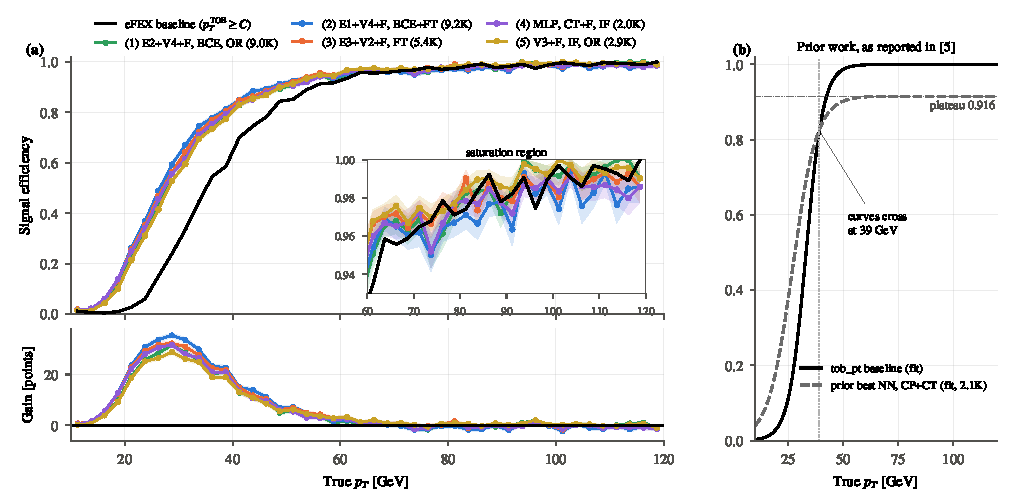
\includegraphics[width=0.97\linewidth]{figures/fig_results_main.pdf}
  \caption{(a) Benchmark turn-ons; model numbers refer to \cref{tab:results_main}. The inset shows saturation, and the lower panel shows gains over the eFEX baseline. Shading indicates statistical uncertainty. (b) Prior-work NN and baseline fits from~\cite{kernan2026}, shown as a separate historical reference. The newly supplied band averages in \cref{tab:results_main} are not point samples of this fit (\cref{app:prior_reference}). Model-name key: \cref{tab:naming}.}
  \label{fig:results_main}
\par\medskip
  \begingroup
  \centering
  \captionof{table}{Benchmark efficiencies [\%] by true-$\pT$ band [GeV]. Red marks our values below the baseline; counts include BatchNorm. The prior-work row is a separately evaluated reference, not part of the ranking. Model-name key: \cref{tab:naming}; provenance: \cref{app:prior_reference}.}
  \label{tab:results_main}
  \small
  \setlength{\tabcolsep}{4pt}
  \begin{tabular}{@{}llrrrrrrr@{}}
\toprule
Criterion & Model & 10--25 & 25--40 & 40--60 & 60--100 & 100--120 & Global & Params \\
\midrule
(1) all bands & E2+V4+\Ffeat, BCE, OR & 14.65 & 62.38 & 88.99 & 97.17 & 99.44 & 67.97$\pm$0.55 & 9.0K \\
(2) global & E1+V4+\Ffeat, BCE+FT & 17.45 & 66.39 & 90.54 & \textcolor{cbred}{96.75} & \textcolor{cbred}{98.28} & 69.61$\pm$0.29 & 9.2K \\
(3) global, $<$6K & E3+V2+\Ffeat, FT & 16.93 & 64.31 & 90.08 & 97.56 & \textcolor{cbred}{98.89} & 69.08$\pm$0.35 & 5.4K \\
(4) global, $<$3K & MLP, \CT+\Ffeat, IF & 16.61 & 62.93 & 89.00 & 97.17 & \textcolor{cbred}{98.53} & 68.40$\pm$0.21 & 2.0K \\
(5) all bands, $<$3K & V3+\Ffeat, IF, OR & 14.13 & 60.42 & 89.14 & 97.89 & 99.50 & 67.47$\pm$0.22 & 2.9K \\
\midrule
--- & Prior best NN, \CP+\CT~\cite{kernan2026} & 12.59 & 60.07 & 86.44 & 90.90 & 91.63 & 62.53 & 2.1K \\
--- & eFEX baseline & 2.28 & 35.85 & 81.60 & 96.89 & 99.34 & 57.37 & --- \\
\bottomrule
\end{tabular}

  \endgroup
\end{figure}

The practical trade-off is clear: all five models turn on earlier, but the highest global efficiency, strongest plateau and smallest network do not coincide. The compact MLP retains much of the CNN gain at less than a quarter of the largest model's size. Seed-level plateau behaviour and the NN-only alternative to the compact OR model are detailed in \cref{app:benchmark_detail}.

% ----------------------------------------------------------------------------
\subsection{What the results tell us}
\label{sec:analysis}
% ----------------------------------------------------------------------------
\Cref{fig:results_analysis} highlights two controlled comparisons. The supporting tables, uncertainties and broader evidence are collected in \cref{app:analysis_weighting,app:analysis_representation,app:analysis_capacity,app:analysis_loss}.



\paragraph{(a) More weight on energetic taus can help.}
The results support the hypothesis in \cref{sec:loss}: emphasising energetic rather than soft taus often helped. Compared with BCE, IF reduced the selected TOB budget (\cref{tab:analysis}). \Cref{fig:results_analysis}a shows the resulting trade-off: after IF training, OR buys a small plateau gain at a larger low-energy cost, so NN-only can win globally. This is input-dependent, not a universal preference for IF or negative $p$ (\cref{app:analysis_weighting}).

\paragraph{(b) Spatial learning and engineered features complement each other.}
CNNs recovered some taus missed by the MLP, consistent with sensitivity to spatial shower patterns. The larger gain came from the fine-grained EM2 input; adding $\Frac$ remained useful, while removing the core convolution retained most performance with fewer parameters (\cref{app:analysis_representation}).

\paragraph{(c) More parameters were not the main route to improvement.}
Wider MLPs and deeper CNNs gave no systematic advantage in the tested families. Similar errors across core-only models point to limited input discrimination rather than insufficient capacity (\cref{app:analysis_capacity}).

\paragraph{(d) The objective controls the trade-off across energies.}
Constrained fine-tuning redistributed efficiency towards protected or rewarded regions, usually with a small global change. The best loss depended on the inputs, and the lowest-energy band remained difficult across methods (\cref{app:analysis_loss}).

% ----------------------------------------------------------------------------
\FloatBarrier
\subsection{Final evaluation of the pair model}
\label{sec:pair_results}
% ----------------------------------------------------------------------------
\paragraph{Seeing two TOBs together improves the turn-on.}
Checkpoints and thresholds were selected on validation and then applied unchanged.
Mean signal efficiency rises from $34.30\%$ to $46.70\%$: a gain of 12.40
percentage points with a seed standard deviation of 0.32 (\cref{tab:pair_final}).
Here signal efficiency is the fraction of signal events that fire; elsewhere
it is the fraction of truth-$\tau$ objects accepted, so the percentages are not
directly comparable. Regional gains, achieved fake rates and the final success
criterion appear in \cref{app:pair_protocol}. The final test does not isolate
which design choice caused the improvement.

\begin{table}[H]
  \centering
  \caption{Final pair-model test efficiencies and achieved event fake rates;
  baseline fake rate: $0.4842\%$. Paired differences use $14{,}509$ signal events.}
  \label{tab:pair_final}
  \small
  \setlength{\tabcolsep}{7pt}
  \begin{tabular}{@{}lrrrr@{}}
\toprule
Seed & Pair model [\%] & Baseline [\%] & Gain [points] & $\FPRev$ [\%] \\
\midrule
42  & 47.07 & 34.30 & 12.77 & 0.5183 \\
123 & 46.55 & 34.30 & 12.25 & 0.5223 \\
456 & 46.48 & 34.30 & 12.19 & 0.5203 \\
\midrule
Mean & 46.70 & 34.30 & $12.40\pm0.32$ SD & 0.5203 \\
\bottomrule
\end{tabular}

\end{table}
